\section{Sistema de Energía (S4)}
La implementación del sistema de energía se reestructuró para alcanzar la estabilidad operativa, separando físicamente la alimentación de la lógica de control de la alimentación de los actuadores de potencia.
\subsection{Implementación del módulo de paro de emergencia (M5)}
\subsubsection{Modificación al módulo de seguridad (paro categoría 0 selectivo)}
Se configuró el botón de paro tipo hongo (NC) para cortar físicamente la alimentación AC exclusivamente de las fuentes de potencia (48V y 24V).

\textbf{Funcionalidad dual implementada:}
\begin{itemize}
	\item \textbf{Corte de potencia (AC):} El bloque de contactos NC interrumpe la fase hacia los drivers, provocando que los motores pierdan par inmediatamente por falta de energía.
	\item \textbf{Señalización (DC):} El botón es alimentado con 3.3V desde la Raspberry Pi. Al presionarse, el cambio de estado es leído por el sistema de control (S7) para detener la lógica del software y alertar al usuario, aunque la Raspberry sigue encendida para mostrar el mensaje.
\end{itemize}

\subsubsection{Verificación del paro de emergencia}
\paragraph*{Prueba S4-02: Desconexión selectiva de potencia.}\mbox{}\\
\textbf{Objetivo:} Verificar que al pulsar el paro, los motores se detienen pero la interfaz se mantiene operativa.
\\
\textbf{Procedimiento:} Con el sistema en movimiento, se presionó el botón de paro.
\\
\textbf{Resultados:}
\begin{itemize}
	\item Las fuentes de 48V y 24V se apagaron completamente.
	\item Los motores se detuvieron por inercia.
	\item La pantalla HMI permaneció encendida, permitiendo visualizar la alerta de seguridad.
\end{itemize}

\subsection{Implementación del módulo de etapa de potencia (M6)}

Se diseñó e implementó un circuito de control de encendido mediante un sistema de enclavamiento con un contactor. El flujo de energía es el siguiente:

\begin{enumerate}
	\item \textbf{Entrada:} La línea de 127 VAC pasa por el fusible principal (M1) hacia un circuito de botones de arranque/paro (Start/Stop) que energizan la bobina de un contactor.
	\item \textbf{Salida del contactor:} Al enclavarse, el contactor habilita la línea de fase principal que se divide en dos ramas:
	\begin{itemize}
		\item \textbf{Rama A (control):} Alimenta directamente al enchufe del eliminador de la Raspberry Pi. Esta rama \textbf{no} pasa por el botón de paro de emergencia, asegurando que el control permanezca encendido mientras el contactor esté activo.
		\item \textbf{Rama B (potencia):} La línea se dirige hacia el botón de paro de emergencia antes de llegar a las fuentes de 24V y 48V.
	\end{itemize}
\end{enumerate}
%% INSERTAR UN DIAGRAMA DE BLOQUES
\subsection{Implementación del módulo de acondicionamiento de energía (M7)}
Debido a los requerimientos de corriente diferenciados, se implementaron tres fuentes independientes:
\begin{itemize}
	\item \textbf{Fuente de potencia alta (48V):} Modelo Mean Well LRS-600-48. Alimenta exclusivamente al driver del motor Nema 34 (abducción).
	\item \textbf{Fuente de potencia media (24V):} Fuente conmutada de 10 A. Alimenta al driver del motor Nema 23 (flexión). Se seleccionó esta capacidad (240W) para tener un amplio margen de seguridad sobre el consumo nominal del motor.
	\item \textbf{Alimentación de control:} Eliminador de pared (AC/DC) conectado a la Raspberry Pi 4. Esta configuración aísla el ruido eléctrico de los motores y garantiza los 3A estables requeridos por el procesador y la pantalla táctil.
\end{itemize}

\subsubsection{Verificación de estabilidad}
\paragraph*{Prueba S4-01: Estabilidad de buses independientes.}\mbox{}\\
\textbf{Resultado:} La separación de fuentes eliminó las caídas de voltaje en la Raspberry Pi que ocurrían al encender los motores en las pruebas preliminares, validando la decisión de emplear tres fuentes.
\clearpage
\section{Sistema de Movimiento (S5)}
La implementación del sistema de movimiento contempló el uso de los motores seleccionados en la etapa de diseño, así como los componentes requeridos para el funcionamiento y control de cada uno. El sistema se compone por dos módulos: M8 y M9, los cuales se describen a continuación. 
\subsection{Implementación del módulo de actuador lineal (M8)}
% Descripción breve: Motor Nema 23, Driver HSS57, sistema de tornillo sin fin/banda.
Comenzando por el módulo correspondiente a la flexión-extensión, la implementación se apegó estrictamente a las especificaciones del diseño detallado, dado que las pruebas de carga preliminares validaron la capacidad del actuador seleccionado.
\begin{itemize}
	\item \textbf{Actuador:} Se instaló el motor a pasos Nema 23 en un control de lazo cerrado con su driver HSS57.
	\item \textbf{Transmisión:} Se realizó el acople del sistema de tornillo sin fin, verificando que no existiera juego mecánico (backlash) que guiara al descarrilamiento del mecanismo.
\end{itemize}

\subsubsection{Verificación del módulo de actuador lineal}
\paragraph*{Prueba S5-01: Desplazamiento lineal y validación de diseño.}\mbox{}\\
\textbf{Objetivo:} Confirmar que el motor Nema 23 es suficiente para desplazar la estructura móvil.
\\
\textbf{Procedimiento:} A través del driver y un código de prueba se activó el motor para realizar el movimiento lineal del mecanismo de flexión-extensión.
\\
\textbf{Resultado:} El mecanismo realiza el recorrido completo de manera fluida. No se requirieron modificaciones al diseño original, validando el cálculo de par inicial para este movimiento.

\subsection{Implementación del módulo de actuador rotativo (M9)}
Durante la fase de integración y pruebas iniciales con carga real (paciente sobre el mecanismo), se encontró que el par del motor Nema 34 ensamblado de forma directa al eje de transmisión no era suficiente para mover la carga. El actuador entraba en estado de fallo al intentar vencer el momento de inercia generado por el peso de la pierna y la fricción del sistema.

\subsubsection{Modificación al diseño del módulo de actuador rotativo}
Para solucionar la falta de potencia, se implementó una modificación técnica que consistió en incorporar una caja reductora planetaria con relación 10:1. Esta elemento tiene como objetivo multiplicar el par de salida del motor, reduciendo velocidad angular, la cual no es requerida para la terapia pasiva lenta, a cambio de la fuerza necesaria para la ejecución del movimiento.

\textbf{Especificaciones del componente integrado:}
\begin{itemize}
	\item \textbf{Tipo:} Reductor planetario para Nema 34 (86 mm).
	\item \textbf{Relación de transmisión:} 10:1.
	\item \textbf{Capacidad de carga:} 30 N.m (nominal) / 50 N.m (máxima).
	\item \textbf{Eficiencia:} 95\% a plena carga.
	\item \textbf{Ventaja operativa:} Aumento del par de retención y lubricación de larga duración.
\end{itemize}
La selección de una relación comercial de 10:1 se basó en una estrategia de diseño robusto. Dado que la aplicación es de terapia pasiva a baja velocidad, se priorizó maximizar el factor de seguridad del par. Una relación de 10:1, con una eficiencia del 95\%, multiplica el par disponible del motor por un factor aproximado de 9.5, logrando con esto mover el mecanismo y realizar el movimiento de abducción-aducción. En la Fig. \ref{fig:dimensiones_caja} se presenta el diagrama dimensional del reductor planetario implementado.

\begin{figure}[h!]
	\centering
	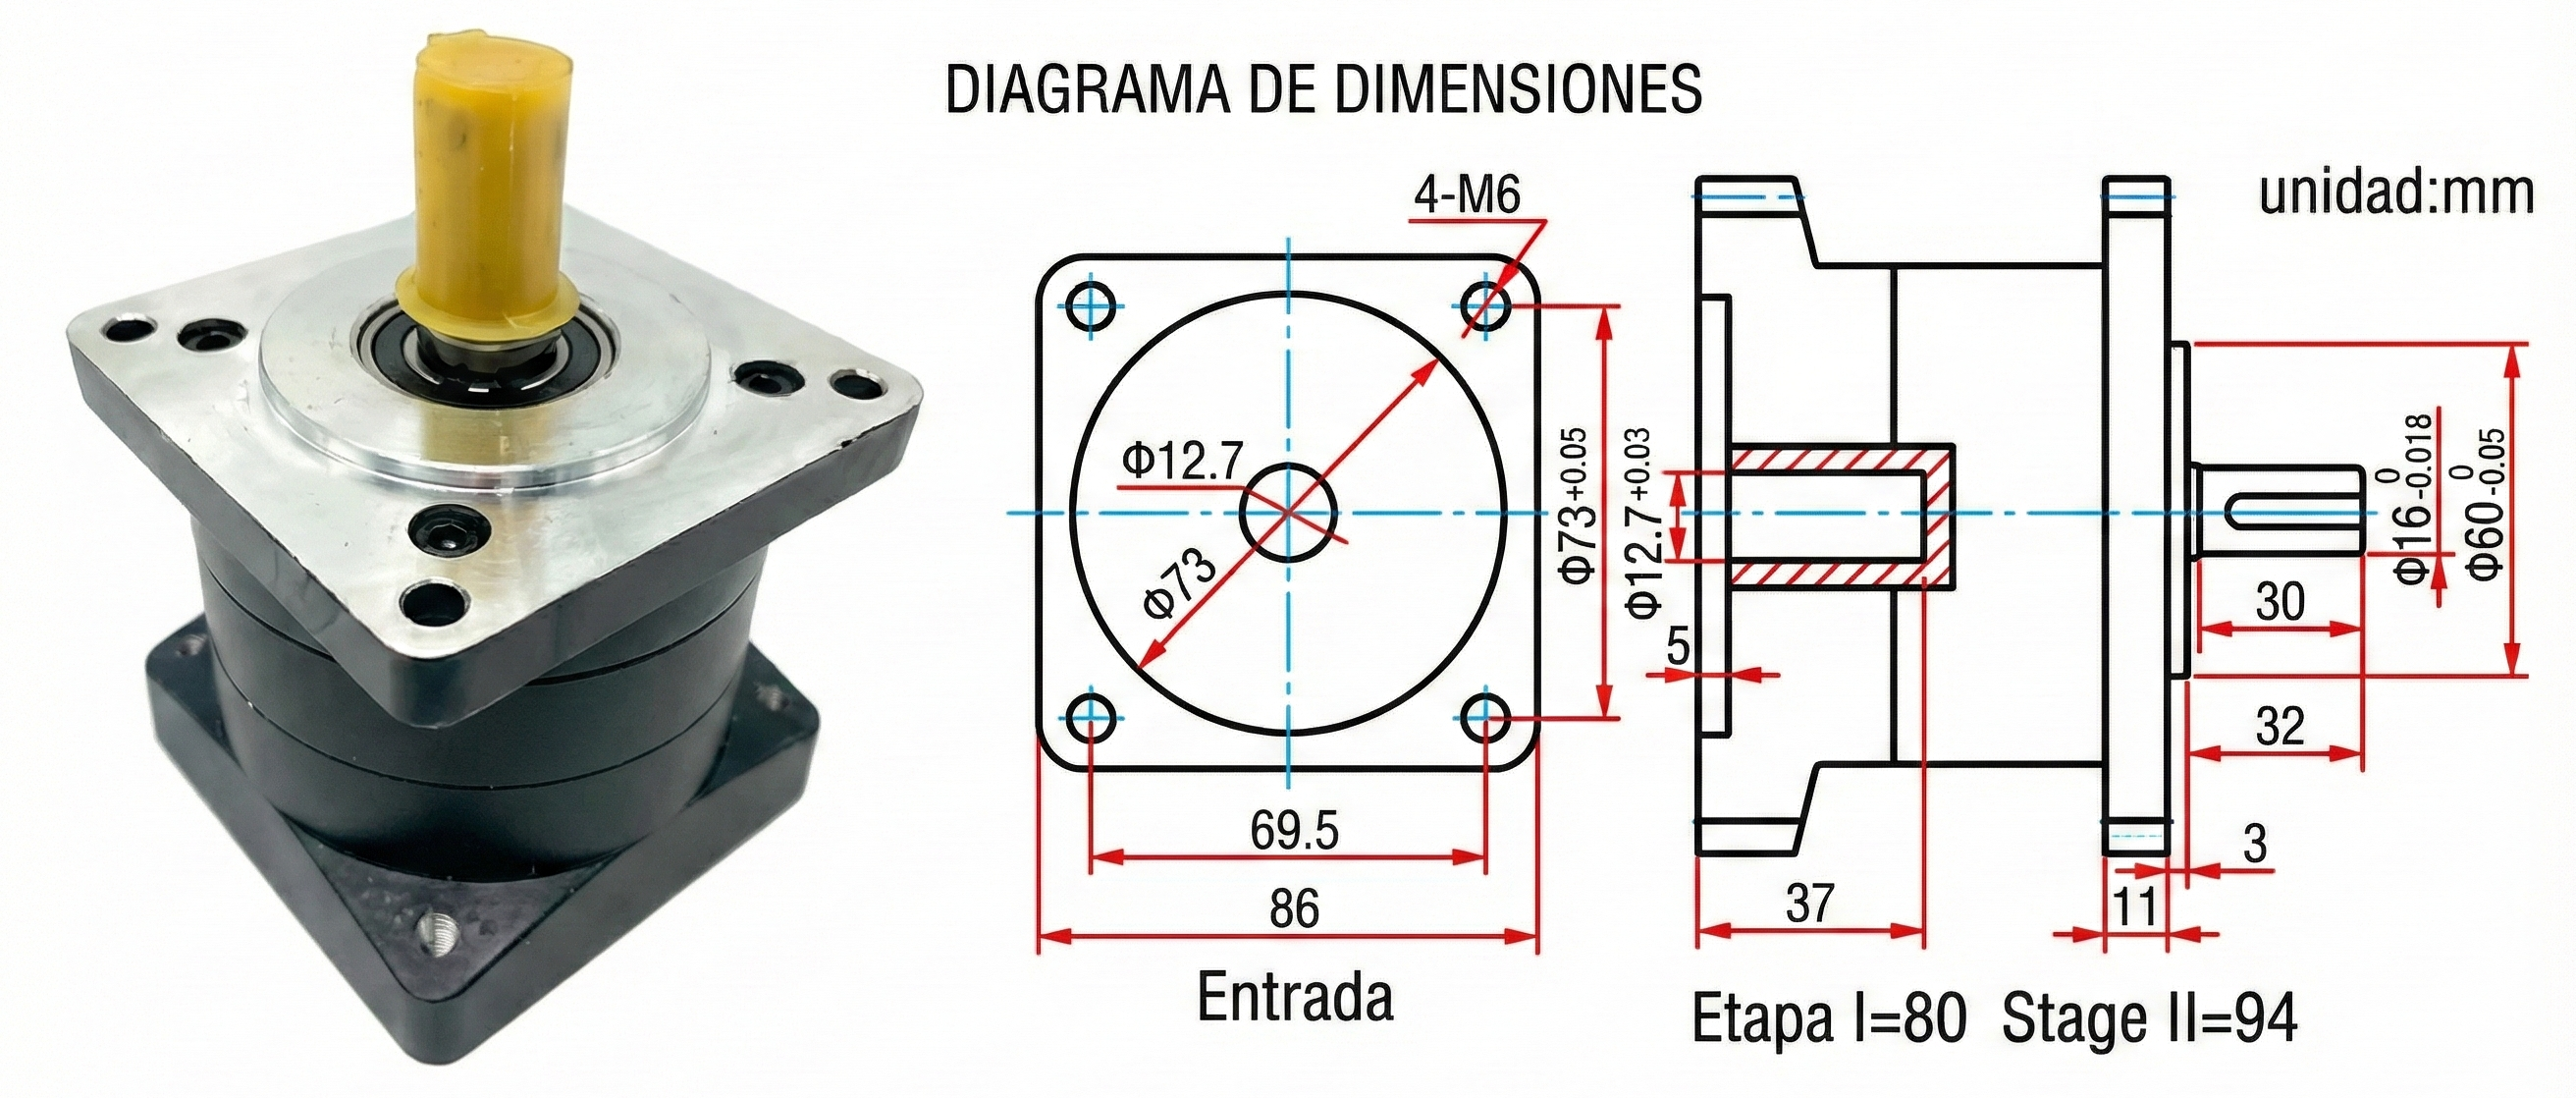
\includegraphics[width=0.9\textwidth]{figure/img_componentes/gearbox_10_1.png}
	\caption{Diagrama dimensional del reductor planetario 10:1 implementado (cotas en mm).}
	\label{fig:dimensiones_caja}
\end{figure}

\subsubsection{Retos de integración y re-manufactura (discrepancia resuelta)}
La incorporación de la caja reductora presentó un desafío de incompatibilidad mecánica: el eje de salida del reductor (16 mm) es de mayor diámetro que el diámetro original maquinado en el eje de transmisión principal del mecanismo de abducción (diseñado originalmente para el eje directo del motor de 14 mm). Esta incompatibilidad requirió una serie de pasos para poder realizar el acople de la caja reductora al eje de transmisión. Dichos pasos se describen a continuación:
\begin{enumerate}
	\item \textbf{Desmontaje:} Se requirió desmontar completamente el subensamble de flexión-extensión (estructura de aluminio) y retirar el eje principal de la estructura de acero.
	\item \textbf{Maquinado de ajuste:} Se llevó el eje de transmisión y las chumaceras a taller para realizar un proceso de barrenado y rectificado, ampliando el diámetro interno para conseguir un ajuste con el nuevo eje de 16 mm de la caja reductora.
	\item \textbf{Alineación:} Durante el re-ensamble, se realizó la alineación de las chumaceras y el eje para lograr transmitir el movimiento desde el motor $\rightarrow$ caja planetaria $\rightarrow$ eje principal, buscando la concentricidad en el ensamble para reducir fricción entre los distintos elementos en esta ruta de transmisión.
\end{enumerate}
En la Fig. \ref{fig:nema34_gearbox} se muestra la integración del reductor planetario al eje de transmisión de potencia para realizar el movimiento de abducción-aducción.
\begin{figure}[h!]
	\centering
	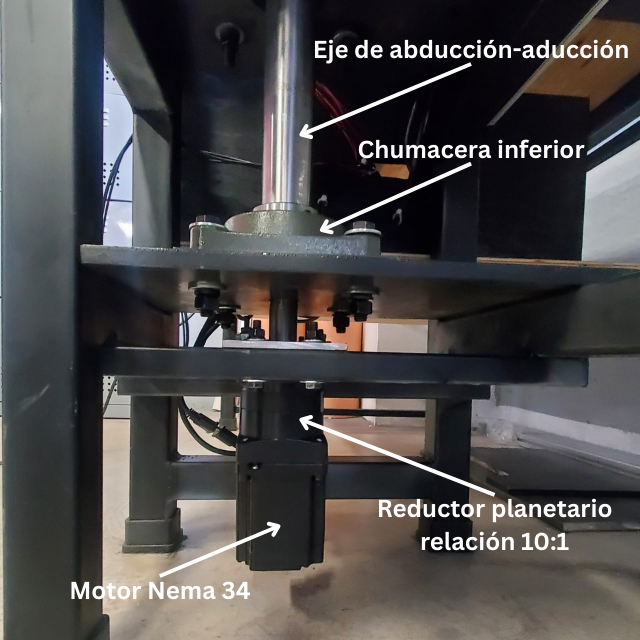
\includegraphics[width=0.5\textwidth]{figure/img_componentes/gearbox.png} 
	\caption{Implementación final del actuador de abducción-aducción con caja reductora planetaria 10:1.}
	\label{fig:nema34_gearbox}
\end{figure}

\subsection{Verificación del módulo de abducción}

\paragraph*{Prueba S5-02: Capacidad de carga con usuario.}\mbox{}\\
\textbf{Objetivo:} Verificar si la relación 10:1 es suficiente para mover la extremidad de un usuario real.
\\
\textbf{Procedimiento:} Se colocó la pierna de un usuario en el mecanismo de flexión-extensión y se comandó el movimiento de abducción.
\\
\textbf{Resultados:} El sistema logró realizar el movimiento de apertura sin pérdida de pasos ni sobrecalentamiento del driver. La inclusión de la caja reductora solucionó el problema de falta de potencia, y el re-maquinado del eje permitió una transmisión de potencia sin deslizamientos.